\section{Automatic Nested Loop Acceleration Framework} \label{sec:acc-framework}
By using a regular SCGRA overlay built on top of the physical FPGA devices, 
we have developed an automatic nested loop acceleration framework targeting 
a hybrid CPU-FPGA system. The goal of the framework is to provide a 
high-productivity nested loop acceleration solution accessible to high-level 
application developers as well as a rapid application-specific 
customization process to achieve better performance-energy trade-off of 
the resulting accelerators. 

\figref{fig:framework} shows the nested loop acceleration framework. Given 
a specified compute intensive loop kernel and high-level design 
goals as well as constraints, the framework automatically 
tunes the design parameters including the SCGRA overlay 
configuration, compilation options and on chip 
communication specifically to the loop kernel through the SCGRA customization 
process. After the customization, corresponding SCGRA overlay based 
FPGA accelerator is generated and implemented through the SCGRA compilation process. 
Meanwhile, the drivers that are needed to utilize the resulting FPGA accelerator 
are generated according to the SCGRA customization. Then the high level application 
is updated and compiled to general purposed processor (GPP) through a 
conventional software compilation process. The application binary code generated in 
combination with the FPGA accelerator bitstream forms the final application 
that will be executed on the hybrid CPU-FPGA system during run time.

\begin{figure}[tb]
\center{\includegraphics[width=0.75\linewidth]{framework}}
\caption{Automatic nested loop acceleration framework}
\label{fig:framework}
\end{figure} 

SCGRA customization process is the focus of this work where optimal 
design choices are decided. Since it involves exploration in a vast 
design space, it is critical to the design productivity of the whole 
framework. In addition, it also determines the configurations of 
the resulting accelerators and thus affects the performance-energy 
trade-off of the final design. In this work, a dedicated customization 
method is proposed to meet both the requirements of the design productivity and 
performance-energy trade-off and it will be further illustrated in the following 
sections.

SCGRA compilation is responsible for mapping the high-level loop 
kernel to the physical FPGA bitstream through a specified SCGRA 
overlay. \figref{fig:horizontal-compilation} presents an overview of the 
compilation process and it includes two compilation flows for two typical
development scenarios i.e. initial compilation and iterated compilation. 
In the first scenario when the specified SCGRA overlay is initially 
implemented on the target physical FPGA device, a standard implementation 
from HDL model may be time-consuming. Fortunately, a hardware-macro compilation 
technique \cite{ROB2014} developed for the regular tiling architectures may 
significantly decrease the implementation time. In the second scenario when 
the specified SCGRA overlay has already been implemented, the bitstream can 
be reused as demonstrated in \cite{scgra} and the compilation can be reduced to seconds.

\begin{figure}[tb]
\center{\includegraphics[width=0.8\linewidth]{horizontal-compilation}}
\caption{High-productivity SCGRA overlay compilation, The whole diagram represents the initial
compilation and it includes both the iterated compilation and the initial implementation.}
\label{fig:horizontal-compilation}
\end{figure}


